\begin{apendicesenv}
  
  \chapter{Processo de Engenharia de Requisitos}
  
    \begin{figure}[!htbp]
      \centering
      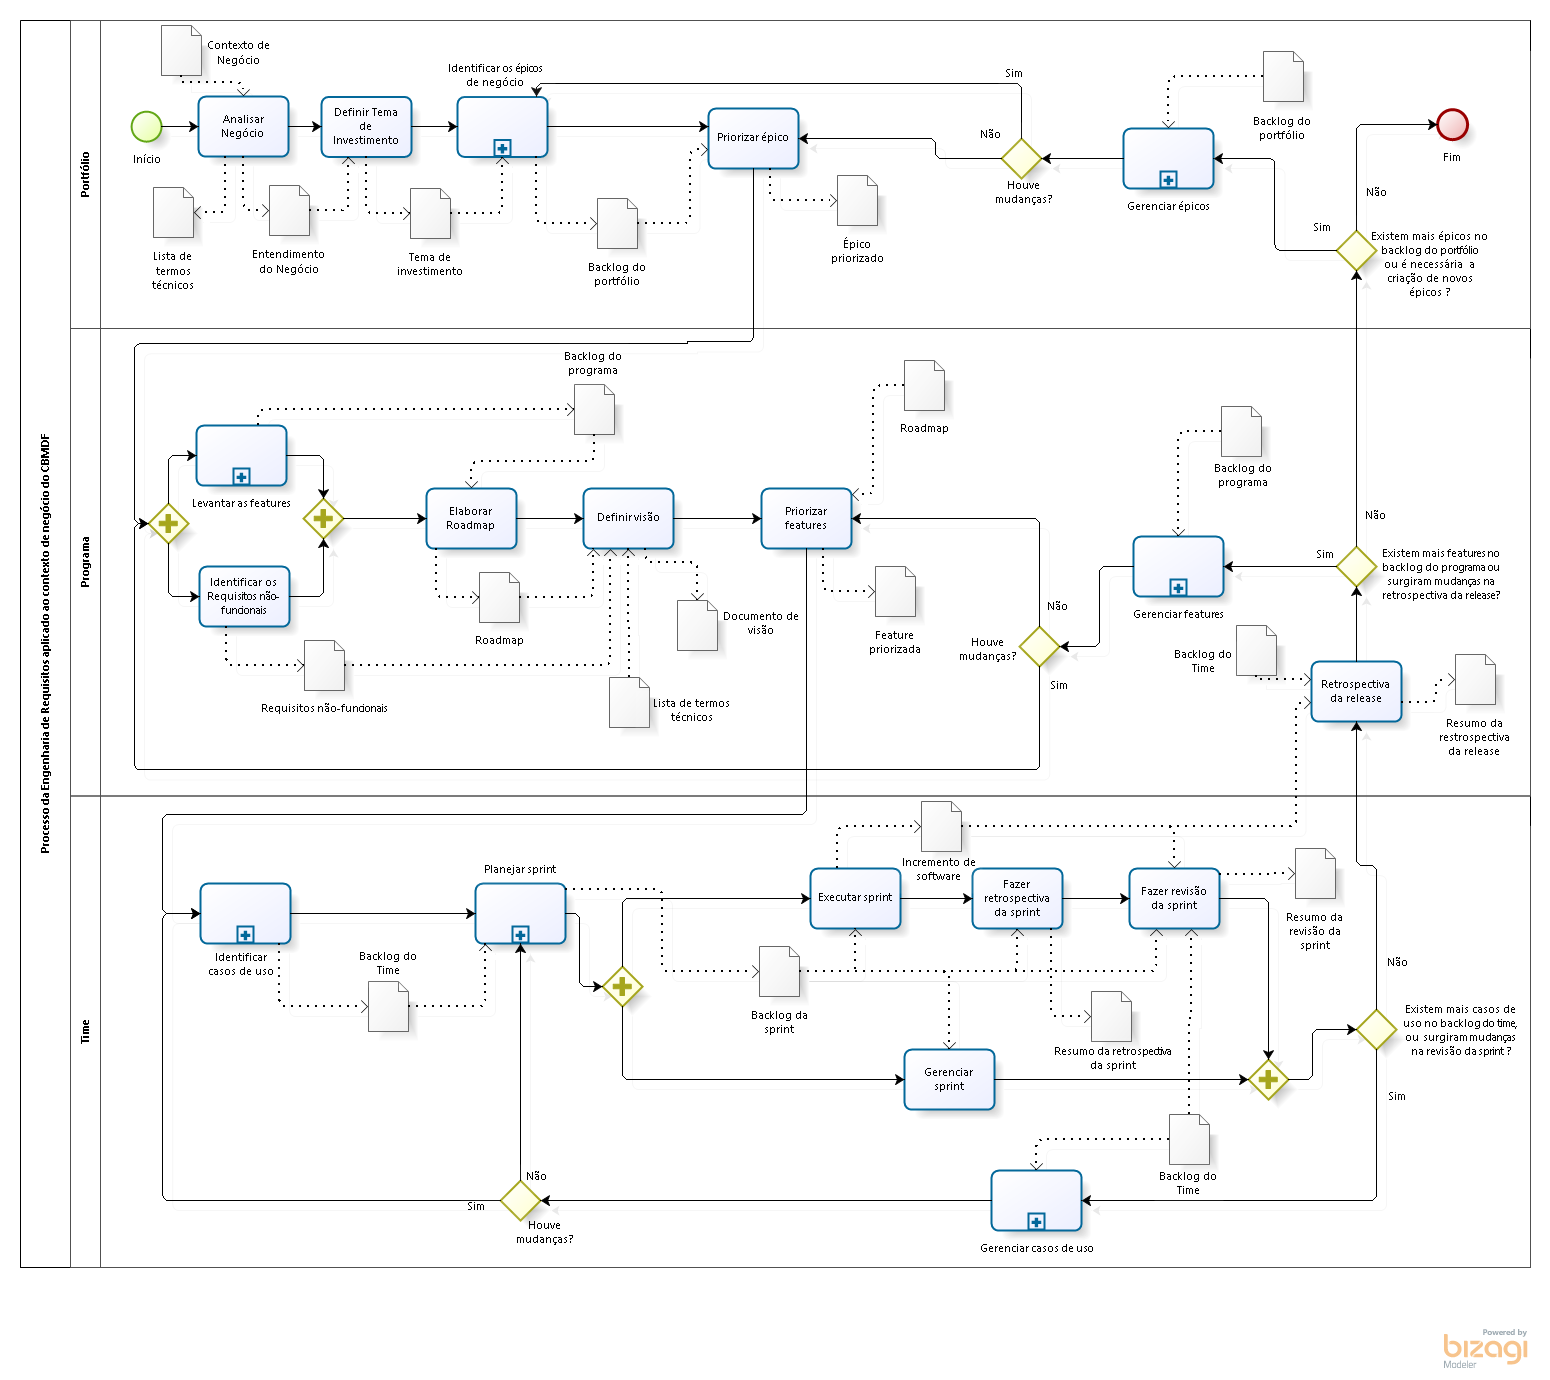
\includegraphics[scale=0.46, angle = 90]{figuras/project_big_picture}
      \caption[Modelo do processo de Engenharia de Requisitos]
	  {Modelo do processo de Engenharia de Requisitos: \textit{Big Picture} do projeto.}
      \label{project_big_picture}
    \end{figure}
  
  \chapter{Documento de visão}

    	{\centering
	\textbf{Corpo de Bombeiros Militar do Distrito Federal}

	\textbf{Documento de visão para o sistema de gerenciamento de viaturas}

	\textbf{2015}

	}
	\textbf{Histórico de Revisões}
	\begin{table}[h]
	\centering
	\label{my-label}
	\begin{tabular}{|l|l|l|l|}
	\hline
	Data & Revisão & Descrição & Autor \\ \hline
	14/06/2015 & 1.0 & Versão Inicial & João Paulo \\ \hline
	22/06/2015 & 1.1 & Adição dos RNF & João Paulo \\ \hline
	     &         &           &       \\ \hline
	\end{tabular}
	\caption{Histórico de Revisões}
	\end{table}
  
	\section{Introdução}
		\subsection{Propósito}
Este documento define as estratégias utilizadas para nortear o desenvolvimento do projeto, 
as necessidades do usuário e envolvidos no projeto,
		\subsection{Resumo da solução}
A solução se apresenta sob a forma de uma aplicação que funcionará na intranet do Corpo de Bombeiros Militar 
do Distrito Federal, e fornecerá subsídios para o correto gerenciamento das viaturas e pessoal relacionado à esse contexto. 
A aplicação será desenvolvida a partir das necessidades do cliente, sem conexão com um sistema legado.
	\section{Descrição do Usuário}
		\subsection{Ambiente de Usuário}
Os usuários são funcionários do Corpo de Bombeiros Militar do Distrito Federal e utilizarão o sistema nas Unidades.
		\subsection{Principais necessidades do Usuário}
Para o usuário é primordial organizar e automatizar a gestão de viaturas e motoristas, 
desde o Departamento de Gestão Veicular até o controle de viaturas e motoristas nas unidades.
	\section{\textit{Stakeholders}}
Os envolvidos no projeto seja no desenvolvimento, na aquisição ou no uso da aplicação final são stakeholders. 
No contexto de desenvolvimento do sistema de gestão de viaturas do CBM-DF temos os seguintes \textit{stakeholders}:
\begin{itemize}
 \item Equipe de desenvolvimento;
 \item Bombeiros do CBM-DF;
 \item Funcionários do DGV;
\end{itemize}
	\section{Resumo do Produto}
Nesta seção serão definidas características do produto.
		\subsection{Perspectiva do Produto}
Espera-se do produto que melhore a gestão de viaturas e motoristas no CBM-DF, facilitando consultas, 
relatórios, verificações e utilização.
		\subsection{Intenção do Produto}
O sistema de gerenciamento automatizará as atividades que hoje são feitas à mão e são arquivadas sob forma de 
planilhas eletrônicas. Os usuários do DGV e Unidades utilizarão o sistema afim de automatizar suas atividades.
		\subsection{Resumo das Capacidades}
O sistema de Gerenciamento de Viaturas e Motoristas do CBM-DF permitirá o gerenciamento de viaturas, 
criando viaturas nos sistemas, alocando viaturas às unidades e modificando os estados das viaturas. 
Também serão gerenciados os motoristas, adicionando os mesmo no sistema, modificando dados do motorista, 
alocando motoristas em escalas e em viaturas.
	\section{Funcionalidades do Produto}
As funcionalidades são um conjunto de características e comportamentos que o sistema deve conter para resolver 
o problema e as necessidades do cliente.
		\subsection{\textit{Feature} 1: Gerenciamento das missões de unidade}
Esta funcionalidade compreenderá comportamentos que permitirão ao usuário fazer gerenciamento de missões 
atribuindo viaturas a elas e gerar relatórios do trabalho registrado no sistema.
		\subsection{\textit{Feature} 2: Gerenciamento dos dados dos abastecimentos das viaturas}
Esta funcionalidade facilitará o gerenciamento dos abastecimentos, visto que o usuário, propriamente dotado de autorização, 
poderá inserir dados de um abastecimento juntamente com o recibo do próprio. Além disso a funcionalidade garante a 
geração de relatórios dos dados aqui contidos.
		\subsection{\textit{Feature} 3: Consulta das viaturas das unidades por dispositivo móvel}
Esta funcionalidade facillitará a consulta de viaturas disponíveis nas unidades e a pesquisa das unidades no mapa. Além disso, 
os dados previamente descritos estarão disponíveis enquanto o dispositivo móvel não estiver conectado à internet.
		\subsection{\textit{Feature} 4: Gerenciamento dos motoristas da unidade}
Esta funcionalidade será empregada tanto para o DGV quanto para as Unidades, com a finalidade de gerenciar o 
motorista desde o cadastro do próprio no sistema quanto na alocação em uma escala e missões, 
além de compreender a geração de relatórios desse assunto.
		\subsection{\textit{Feature} 5: Gerenciamento das viaturas da unidade}
Esta funcionalidade compreende as necessidades do usuário de gerenciar viaturas desde o cadastro e alocação, 
até o desígnio para as missões. Aterações de estado e geração de relatórios deste assunto estão aqui contidos.

	\section{Requisitos não-funcionais}		
Requisitos não-funcionais são regras que, mesmo não sendo funcionalidades, o sistema deve estar de acordo. Para o contexto do 
sistema de gerenciamento de viaturas os seguintes requisitos não-funcionais foram identificados:
\begin{itemize}
 \item O sistema deve ficar online 24/7;
 \item O sistema deve estar disponível na Intranet do CBMDF;
 \item O sistema deve possuir uma interface autoexplicativa;
 \item O sistema deve fornecer informações mais detalhadas sobre o funcionamento de suas funcionalidades, quando necessário;
 \item O sistema deve possuir uma versão mobile, com determinadas funcionalidades, na plataforma Android;
 \item O sistema deve manter uma cópia local e atualizada de determinados dados, em sua versão mobile, provenientes do banco de dados do sistema;
 \item O sistema deve exigir uma verificação de identidade para que o acesso seja liberado.
\end{itemize}
	\section{Documentação dos Requisitos}
		\subsection{Glossário}
Neste item definimos termos a fim de tornar comum o entendimento dos envolvidos.
\begin{itemize}
 \item \textit{Stakeholder}: Envolvido com a produção,utilização ou gerenciamento do projeto.
 \item CBM-DF: Corpo de Bombeiros Militar do Distrito Federal.
 \item DGV: Departamento de Gestão Veicular.
 \item Chamado: Demanda criada por uma ligação de telefone e passada pela central para alguma unidade.
 \item Missão: Atividade dos bombeiros das unidades.
\end{itemize}


  \chapter{Especificação Casos de Uso}
  
    \label{Especificacao}
      \subsection{Caso de Uso F1UC1 - Cadastrar Missão}

  {\raggedright
      \textbf{Descrição}
  }
  
    Este caso de uso permite que o Sargento cadastre uma missão do Corpo de Bombeiros do Distrito Federal (CBMDF)  para manter o registro desta no sistema.    
  
  {\raggedright
      \textbf{Ator Principal}
  }

    Sargento. O Sargento é a patente responsável pela Gestão Operacional da corporação do Corpo de Bombeiros do Distrito Federal (CBMDF).
  
  {\raggedright
      \textbf{Fluxo Principal}
  }
  
    Este caso de uso é iniciado quando o Sargento escolhe a opção de cadastrar missão.
  
  \begin{enumerate}
  \item O sistema solicita ao Sargento que sejam adicionados dados da missão. 
  \item O Sargento preenche as informações e solicita a confirmação de cadastro.
  \item O sistema faz a validação dos dados preenchidos. [RN01][RN02][FE01]
  \item O sistema apresenta os dados informados para confirmar o cadastro.
  \item O Sargento confirma a inclusão. 
  \item O sistema cadastra a missão.
  \item O sistema informa uma mensagem de confirmação do cadastro da missão.[PE01].
  \item O caso de uso é encerrado.
  \end{enumerate}
  
  \pagebreak
  
   {\raggedright
      \textbf{Regras de Negócio}
   }
   
   \textbf{RN01} – Validação das informações.
   
   A Tabela a seguir apresenta os dados do motorista que devem ser validados.
   
   \begin{table*}[!h]
    \centering
      \begin{tabular}{|p{0.20\linewidth}|p{0.25\linewidth}|p{0.20\linewidth}|p{0.20\linewidth}|}
      \hline
      Campo  & Formato & Valores & Obrigatoriedade\\
      \hline

      Tipo de viatura & - & Terrestre, aquático e aéreo & Sim\\ \hline

      Viatura & - & - & Sim\\\hline
      
      Motorista & - & - & Sim\\\hline
      
      Tipo de missão & - & - & Sim\\\hline
      
      \textit{Status} da missão & - & Em andamento, finalizada & Sim\\\hline
      
      Descrição & - & - & Sim\\\hline
      
      Local da missão & - & - & Sim\\\hline
      
      \hline
      \end{tabular}
    \end{table*}

    \textbf{RN02} – Identificador da missão.
    O identificador da missão é um número com auto-incremento.
    
   {\raggedright
      \textbf{Fluxo de Exceção}
   }
   
   FE01. Validação de dados
	No passo 3 do fluxo principal, é verificado pelo sistema que um ou mais campos não foram validados (no formato e/ou
	obrigatoriedade de preenchimento). O sistema exibe uma mensagem informando o ocorrido ao Gestor Administrativo e retorna
	ao passo 1 do fluxo principal.

	
   {\raggedright
      \textbf{Condições}
   }
   
    
   \textbf{Pré-condições}
   
   O Sargento deve estar corretamente autenticado no sistema para a execução do caso de uso.
   
   \textbf{Pós-condição}
   
   A operação realizada no caso de uso deve ser registrada, juntamente com o autor, data e horário da operação, para fins de auditorias futuras.
   
   \textbf{Ponto de extensão}
   
   PE01. Incluir o caso de uso: Associar motorista a viatura.
   No passo 7 do fluxo principal, o caso de uso F4UC9 - Gerenciar vínculo entre motoristas e viaturas deve ser executado.
      \section{Caso de Uso F1UC2 - Alterar Missão}

  {\raggedright
      \textbf{Descrição}
  }
  
    Este caso de uso permite ao Sargento alterar os dados de uma missão previamente cadastrada no sistema de gerenciamento de viaturas do CBMDF.

  {\raggedright
      \textbf{Ator Principal}
  }

    Sargento. O Sargento é a patente responsável pela Gestão Operacional da corporação do Corpo de Bombeiros do Distrito Federal (CBMDF).
  
  {\raggedright
      \textbf{Fluxo Principal}
  }
  
    Este caso de uso é iniciado quando o Sargento escolhe a opção de alteração de dados da missão.
    
  \begin{enumerate}
  \item O sistema solicita ao Sargento que informe a missão que deseja-se ter os dados alterados.
  \item O Sargento informa os dados da missão pelos quais deseja fazer a pesquisa e solicita a consulta. [PE01]
  \item O sistema apresenta os dados da missão solicitada e permite a edição.[RN01]
  \item O Sargento realiza as mudanças necessárias e solicita a alteração.
  \item O sistema faz a validação dos dados preenchidos.  [FE01]
  \item O sistema apresenta os dados informados para confirmação da alteração.
  \item O Sargento confirma a alteração dos dados da missão.
  \item O sistema altera os dados da missão.
  \item O sistema apresenta uma mensagem de confirmação da alteração.
  \item O caso de uso é encerrado.
  \end{enumerate}
  
  \pagebreak
  
   {\raggedright
      \textbf{Regras de Negócio}
   }
   
   \textbf{RN01} – Dados que podem ser alterados.
   
   A Tabela a seguir apresenta os dados da missão que podem ser alterados.
   
   \begin{table*}[!h]
    \centering
      \begin{tabular}{|p{0.20\linewidth}|p{0.25\linewidth}|p{0.20\linewidth}|p{0.20\linewidth}|}
      \hline
      Campo  & Formato & Valores & Obrigatoriedade\\
      \hline

      \textit{Status} da missão & - & Em andamento, finalizada & Sim\\\hline
      
      Descrição & - & - & Sim\\\hline
      
      \hline
      \end{tabular}
    \end{table*}

   {\raggedright
      \textbf{Fluxo de Exceção}
   }
   
   FE01. Validação de dados
	No passo 5 do fluxo principal, é verificado pelo sistema que um ou mais campos não foram validados (no formato e/ou
	obrigatoriedade de preenchimento). O sistema exibe uma mensagem informando o ocorrido ao Gestor Administrativo e retorna
	ao passo 1 do fluxo principal.

	
   {\raggedright
      \textbf{Condições}
   }
   
    
   \textbf{Pré-condições}
   
   O Sargento afim de realizar o cadastro da missão deve estar devidamente autenticado no sistema para a execução do caso de uso.

   \textbf{Pós-condição}
   
   A operação realizada no caso de uso deve ser registrada, juntamente com o autor, data e horário da operação, para fins de auditorias futuras.
   
   \textbf{Ponto de extensão}
   
   PE01. Incluir o caso de uso: Consultar missão.
   No passo 2 do fluxo principal, o caso de uso F1UC3 - Consultar missão deve ser executado.
      \section{Caso de Uso F1UC3 - Consultar Missão}

  {\raggedright
      \textbf{Descrição}
  }
  
    Este caso de uso permite que o Consultor operacional consulte missões da corporação do Corpo de Bombeiros do Distrito Federal (CBMDF) para ter acesso as informações da(s) mesma(s).
  
  {\raggedright
      \textbf{Ator Principal}
  }

    Consultor Operacional.
  
  {\raggedright
      \textbf{Fluxo Principal}
  }
  
    Este caso de uso é iniciado quando o consultor operacional escolhe a opção de consultar  missão(ões).
    
  \begin{enumerate}
  \item O sistema solicita ao consultor operacional que informe os dados pelos quais deseja-se consultar a(s) missão(ões).
  \item O consultor operacional informa os dados da missão pelos quais deseja fazer a pesquisa e solicita a consulta. [RN01][FE01]
  \item O sistema apresenta os dados da(s) missão(ões) solicitada(s).[FE02][RN02]
  \item O caso de uso é encerrado .
  \end{enumerate}
  
   {\raggedright
      \textbf{Regras de Negócio}
   }
   
   \textbf{RN01} – Parâmetros de pesquisa.
   
   A Tabela a seguir apresenta os parâmetros para pesquisa de motorista(s).

   \begin{table*}[!h]
    \centering
      \begin{tabular}{|p{0.20\linewidth}|p{0.25\linewidth}|p{0.20\linewidth}|p{0.20\linewidth}|}
      \hline
      Campo  & Formato & Valores & Obrigatoriedade*\\
      \hline

      Tipo de missão por unidade** & - & Em andamento, finalizada & Sim\\\hline
      
      Tipo de missão & - & - & Sim\\\hline
      
      \textit{Stauts} da missão & - & Em andamento, finalizada & Sim\\\hline
      
      \hline
      \end{tabular}
    \end{table*}
      
      *Pelo menos um dos parâmetros deve ser preenchido.
      ** Apenas o DGV poderá pesquisar por unidade.
   
   \textbf{RN02} – Restrição de visualização.
   
   Para o DGV a consulta pode apresentar todas as missões do Corpo de Bombeiros do Distrito Federal (CBMDF).
   
   {\raggedright
      \textbf{Fluxo de Exceção}
   }
   
   FE01. Validação de dados
	No passo 2 do fluxo principal, é verificado pelo sistema que um ou mais campos não foram validados (no formato e/ou
	obrigatoriedade de preenchimento). O sistema exibe uma mensagem informando o ocorrido ao Gestor Administrativo e retorna
	ao passo 1 do fluxo principal.

	
   {\raggedright
      \textbf{Condições}
   }
   
    
   \textbf{Pré-condições}
   
   O consultor operacional deve estar corretamente autenticado no sistema para a execução do caso de uso.
   
   \textbf{Pós-condição}
   
   A operação realizada no caso de uso deve ser registrada, juntamente com o autor, data e horário da operação, para fins de auditorias futuras.
   
   \textbf{Ponto de extensão}
   
   PE01. Incluir o caso de uso: Consultar missão.
   No passo 2 do fluxo principal, o caso de uso F1UC3 - Consultar missão deve ser executado.
    
  \section{Caso de Uso F4UC5 - Cadastrar motorista}

  {\raggedright
      \textbf{Descrição}
  }

    Este caso de uso permite que o Gestor Administrativo cadastre um motorista na corporação do Corpo de Bombeiros do Distrito Federal
    (CBMDF) para manter o registro deste no sistema.
    
  {\raggedright
      \textbf{Ator Principal}
  }

    Gestor Administrativo. O Gestor Administrativo representa os Tenentes e Capitães da corporação do Corpo de Bombeiros do Distrito
    Federal (CBMDF).

  {\raggedright
      \textbf{Fluxo Principal}
  }
  
    Este caso de uso é iniciado quando o Gestor Administrativo escolhe a opção de cadastrar um motorista na corporação.
    
  
  \begin{enumerate}
    \item O sistema solicita ao Gestor Administrativo o preenchimento dos dados de um motorista.
    \item O Gestor Administrativo preenche os dados e solicita a confirmação de cadastro.
    \item O sistema faz a validação dos dados preenchidos.[RN01][FE01]
    \item O sistema apresenta os dados informados para confirmação do cadastro.
    \item O Gestor Administrativo confirma a inclusão do motorista.
    \item O sistema cadastra o motorista informado.
    \item O sistema apresenta uma mensagem de confirmação do cadastro.
    \item O caso de uso é encerrado.
    
  \end{enumerate}
  
  
   {\raggedright
      \textbf{Regras de Negócio}
   }
   
   \textbf{RN01} – Validação das informações.
   
   A Tabela a seguir apresenta os dados do motorista que devem ser validados.
   
   \begin{table*}[!h]
    \centering
      \begin{tabular}{|p{0.20\linewidth}|p{0.25\linewidth}|p{0.20\linewidth}|p{0.20\linewidth}|}
      \hline
      Campo  & Formato & Valores & Obrigatoriedade\\
      \hline

      Matrícula do motorista & 000000/0 & - & Sim\\ \hline

      Patente do motorista & - & - & Sim\\\hline
      
      Curso de especialização & - & - & Sim\\\hline
      
      Curso de especialização & - & - & Sim\\\hline
      
      Ano do curso de especialização & 0000 & - & Sim\\\hline
      
      Número da CNH & - & - & Sim\\\hline
      
      Número da CNH & - & A, B, C, D e E & Sim\\\hline
      
      Data de Vencimento da CNH & 00/00/0000 & - & Sim\\\hline
      
      \hline
      \end{tabular}
    \end{table*}

    \pagebreak
    
   {\raggedright
      \textbf{Fluxo de Exceção}
   }
   
   FE01. Validação de dados
	No passo 3 do fluxo principal, é verificado pelo sistema que um ou mais campos não foram validados (no formato e/ou
	obrigatoriedade de preenchimento). O sistema exibe uma mensagem informando o ocorrido ao Gestor Administrativo e retorna
	ao passo 1 do fluxo principal.

	
   {\raggedright
      \textbf{Condições}
   }
   
    
   \textbf{Pré-condições}
   
   O Gestor Administrativo deve estar corretamente autenticado no sistema para a execução do caso de uso.
   
   \textbf{Pós-condição}
   
   A operação realizada no caso de uso deve ser registrada, juntamente com o autor, data e horário da operação, para fins de auditorias futuras.




  
  
  
\end{apendicesenv}
